\newpage
\subsection{Implementing grow}
\visHeader
\hypertarget{growBox vis}{}

\begin{itemize}
 
\item[$\blacktriangleright$] Start by creating the simple story pattern depicted in Fig.~\ref{fig:sdm_grow_1}. This matches the box
(\texttt{this}), with \emph{any} two partitions in the box\footnote{Remember, this is for the \emph{pattern matcher}}.

\begin{figure}[htbp]
\begin{center}
  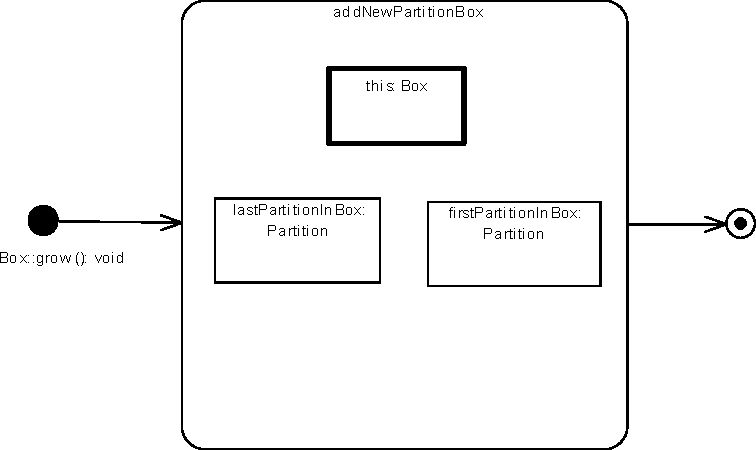
\includegraphics[width=\textwidth]{ea_elementsGrowBox.pdf}
  \caption{Context elements for SDM}  
  \label{fig:sdm_grow_1}
\end{center}
\end{figure}

\item[$\blacktriangleright$] To create the appropriate \mbox{NAC} (to constrain the possible matches for \texttt{lastPartitionInBox}),  create the new object
variable \texttt{nextPartition}, of type \texttt{Partition}, and set \note{Binding Semantics} its \emph{Binding Semantics} to \texttt{negative}
(Fig.~\ref{fig:sdm_grow_2}). The object variable should be visualised as being cancelled or struck out. % why?
 
\begin{figure}[htbp]
\begin{center}
  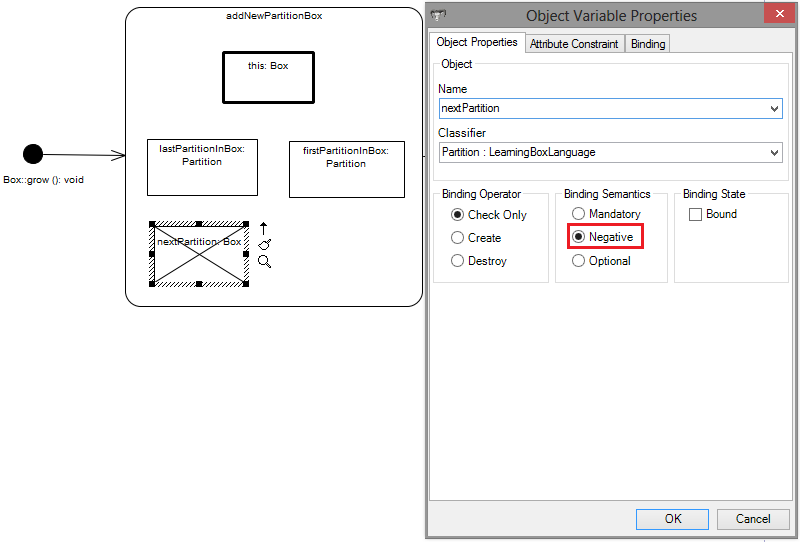
\includegraphics[width=0.9\textwidth]{ea_negElement}
  \caption{Adding a negative element}  
  \label{fig:sdm_grow_2}
\end{center}
\end{figure}
 
\item[$\blacktriangleright$] Now, quick link \texttt{nextPartition} to \texttt{lastPartitionInBox}, but be sure choose the link type carefully! The
\texttt{nextPartition} should play the role of \texttt{next} with respect to \texttt{lastPartitionInBox}.

\item[$\blacktriangleright$] Complete the story pattern so that it closely resembles Fig.~\ref{fig:sdm_grow_3}. 

\begin{figure}[htbp]
\begin{center}
  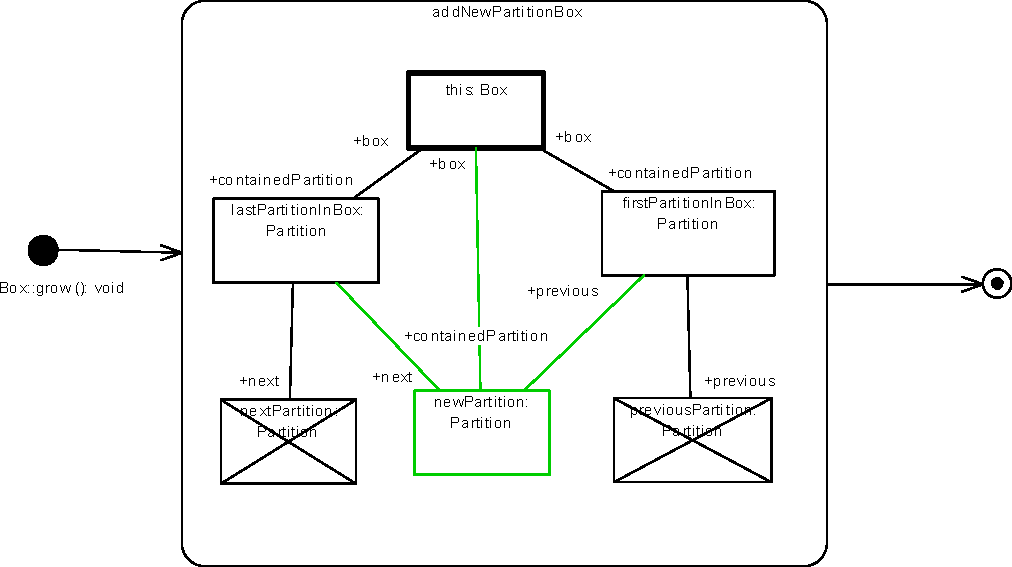
\includegraphics[width=\textwidth]{ea_NACFirstLast.pdf} 
  \caption{Determining the first and last partition with NACs}  
  \label{fig:sdm_grow_3}
\end{center}
\end{figure}
 
\item[$\blacktriangleright$] Notice how the created partition \texttt{newPartition} is `hung' into the box. It becomes the next partition of the current
\emph{last} partition, and has its previous partition set to the first partition in the box (as depicted with the arrows in Fig.~\ref{fig:membox_depiction}).
  
\item[$\blacktriangleright$] To complete this SDM, build the assignment to set the size of the new partition. Go ahead and invoke the corresponding dialogue to
activate the \texttt{:=} operator.

Given that the new size must be calculated using a helper function via a \emph{MethodCallExpression}.\define{MethodCallExpression}A MethodCallExpression is
used to invoke a method defined in any class in the current EA project. Enter the values in Fig.~\ref{fig:sdm_grow_4}, choosing the argument \texttt{this} as
the target, and \texttt{determineNextSize} as the method to be invoked. 

Since \texttt{determineNextSize} doesn't require any parameters, you can ignore the \texttt{Parameters} field this time, but for future reference, parameters
can be specified by choosing the appropriate parameter declaration between guillemets (e.g. \texttt{<Box box>}) found in the drop-down menu and typing in the
value (this is basically a literal expression). Don't forget to press the \texttt{Save} button for every parameter, then \texttt{Add} + \texttt{OK} to confirm
and close the dialogue.
 
 %UPDATE not under 'target' but 'objects'
\begin{figure}[htbp]
\begin{center}
  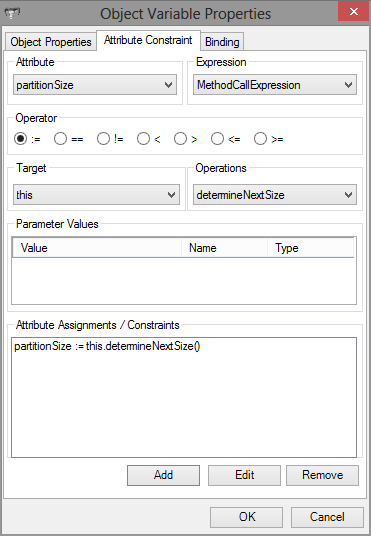
\includegraphics[width=0.5\textwidth]{ea_methodCall.png}
  \caption{Invoking a method via a \texttt{MethodCallExpression} {\bf UPDATE}}  
  \label{fig:sdm_grow_4} 
\end{center}
\end{figure}

\item[$\blacktriangleright$]  If you've done everything right, your SDM should now closely resemble Fig.~\ref{fig:sdm_grow_5}. 

% As usual, try to export, generate code, inspect the
% method implementation and write a JUnit test.  This time around you also have to
% implement the helper method \texttt{determineNextSize} directly in the
% generated code
% (\texttt{gen/\-LearningBoxLanguage/\-facade/\-impl/\-LearningBoxUtilImpl}).
% Don't forget to add \texttt{@generated NOT} to the Java doc comment of the
% method so the code generator preserves your code in future runs.
% When testing (which you will \emph{of course} do right?), note that you can only grow a ``minimal'' box that has at least a first and last partition, i.e., a box with 
%no partitions at all cannot be grown using our specified SDM. 

\begin{figure}[htbp]
\begin{center}
  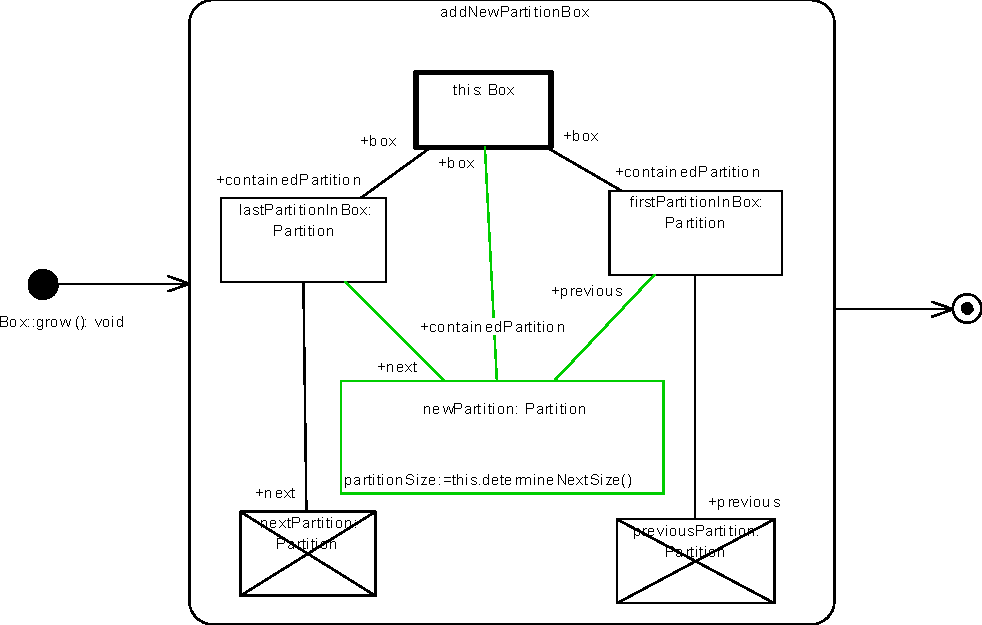
\includegraphics[width=0.9\textwidth]{ea_completeActivityGrowBox.pdf}
  \caption{Complete SDM for \texttt{Box::grow}}  
  \label{fig:sdm_grow_5}
\end{center}
\end{figure}

\item[$\blacktriangleright$]  That's it - your \texttt{grow} SDM is complete! This was probably the most challenging SDM to build, so give yourself a solid 
pat on the back. If you found it easy then \ldots gee whiz, I don't think i'm doing my job correctly. To see how this is done in the texual syntax, review
Fig.~\ref{fig:patternComplete}.\footnote{We do recommend reading the instructions for this one, however, since NACs can be tricky.}

\end{itemize}
